%\documentclass{beamer}
\documentclass[handout]{beamer}

\usepackage{pgfpages} 

%\setbeameroption{show only notes}

\usetheme{default}

\mode<presentation> {
%  \usetheme{Warsaw}
  \usetheme{Frankfurt}
%  \usetheme{Boadilla}
%  \usetheme{Marburg}
}

\mode<handout>{\setbeamercolor{background canvas}{bg=black!5} %
    \pgfpagesuselayout{4 on 1}[letterpaper,border shrink=4mm,landscape] %
    \setbeameroption{show notes}}

\title[CAC Intro] {An Introduction to\\ The Center for Advanced Computing}
\author{Brock Palen\\ \texttt{brockp@umich.edu}}
\date{TBD}

\begin{document}
  \setbeamercovered{transparent}  
  \begin{frame}
    \titlepage
    \url{http://cac.engin.umich.edu/training}
  \end{frame}

%table of contents
  \begin{frame}{Outline}
    \tableofcontents
  \end{frame}
  
  \section{Resources}
  \subsection {TeraGrid}
  \begin{frame}{TeraGrid}
   \begin{block}{About}
"TeraGrid is an open scientific discovery infrastructure combining leadership class resources at eleven partner sites to create an integrated, persistent computational resource."
   \end{block}
   \begin{block}{Getting Started}
    \begin{itemize}
     \item Visit \url{http://cac.engin.umich.edu/teragrid/}
     \item Schedule an appointment with the CAC staff about getting an allocation and which resources are right for you
     \item Questions go to \url{tg-support@umich.edu}
    \end{itemize}
   \end{block}
   \note{
       TeraGrid integrates high-performance computers, data resources and tools. Currently, TeraGrid resources include more than a petaflop of computing capability and more than 30 petabytes of online and archival data storage. Researchers can also access more than 100 discipline-specific databases. 
\\
TeraGrid is for users who need access to resources that can not be provided on campus. This would be users who need access to very large parallel jobs, huge amounts of total jobs, or large data access and visualization.

   } % end note
  \end{frame}

  \subsection {Hardware}

  \begin{frame}{Hardware}
   \begin{block}{Compute Hardware}
    \begin{itemize}
    \item 1 Altix node, 32 cores
    \item 800 Compute nodes, over 4600 cores
    \item Gigabit networking and Infiniband networking
    \item Upto 96GB of memory (64GB public) for SMP work
    \end{itemize}
   \end{block}
   \begin{block}{Visualization Hardware}
    \begin{itemize}
     \item \url{http://um3d.dc.umich.edu/}
     \item Windows 64bit Nvidia 8GB Quad Core
     \item Linux Nvidia 16GB Quad Core 30" wide screen
    \end{itemize}
   \end{block}
  \end{frame}
%nyx
  \begin{frame}{Hardware: nyx}
   \begin{columns}[c]
   \begin{column}{7cm}
    \begin{block}{Nyx}
    \begin{itemize}
    \item nyx is the Opteron cluster;
    \item Login: \texttt{nyx-login.engin.umich.edu}
    \item Running RedHat Enterprise Linux 5
    \item Uses PBS for Resource Access
    \item Logins only allowed from on campus addresses
    \item Logins allowed when connected via the ITS VPN Service \url{http://www.itcom.itcs.umich.edu/vpn/}
    \end{itemize}
   \end{block}
   \end{column}
   \begin{column}{5cm}
    \begin{center}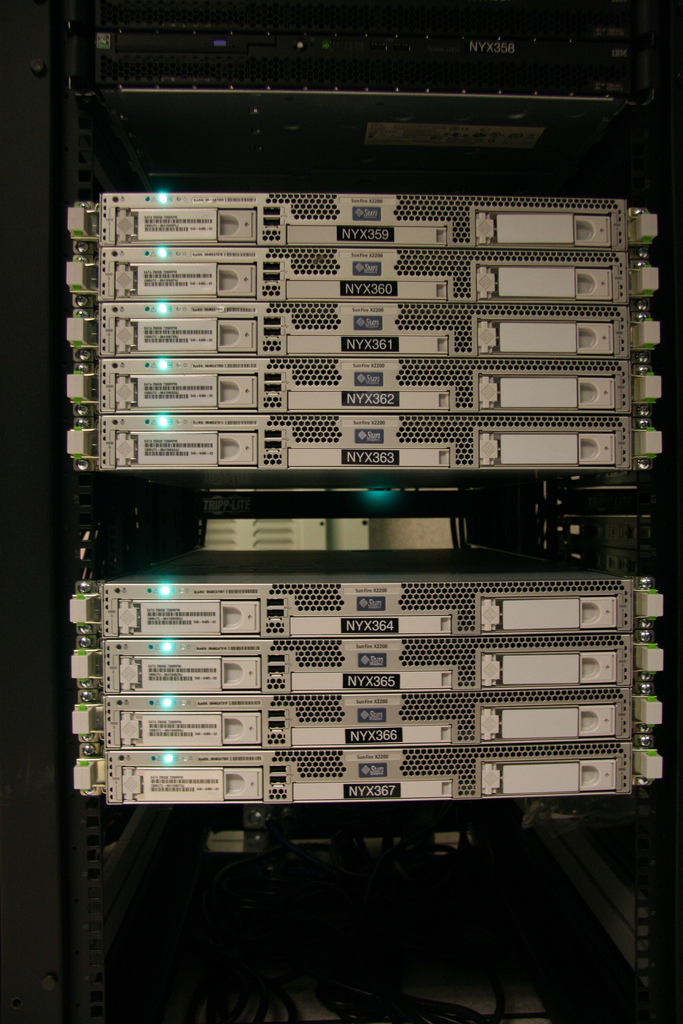
\includegraphics[height=2.7in]{nyx}\end{center}
   \end{column}
  \end{columns}
  \end{frame}
%nyx-login pools
  \begin{frame}{Hardware: nyx-login}
   \begin{center}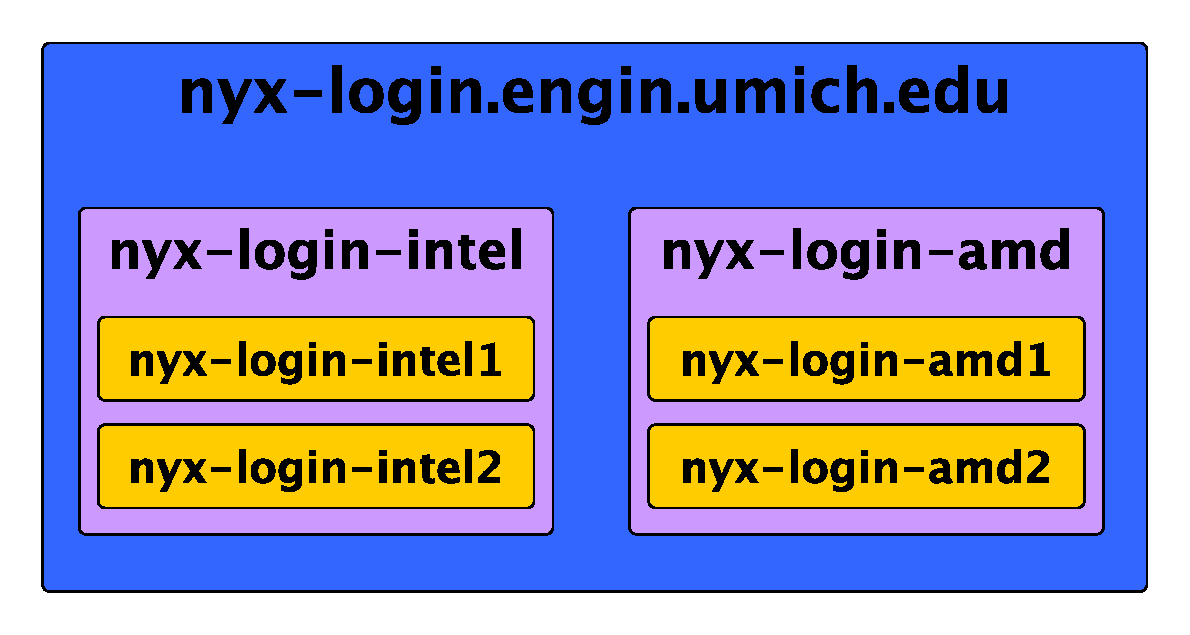
\includegraphics[height=2.5in]{nyx-login}\end{center}
  \end{frame}
%note
   \note{\texttt{nyx-login.engin.umich.edu} is a pool of currently 5 machines (subject to change). When you first connect the login session will go to one of the 5 nodes randomly. Future sessions from that machine for the day should go to the same machine.  You can check the specific machine the session is on by running \texttt{hostname}. The 5 machines are split between the two types of systems the nyx cluster supports currently AMD and Intel.  If you do not care the type of login node you land on (matlab, abaqus etc) use \texttt{nyx-login.engin.umich.edu}.  If the type of machine is of interest use \texttt{nyx-login-intel.engin.umich.edu} or \texttt{nyx-login-amd.engin.umich.edu}.  These pools contain only login nodes of that type.  Note that cpu models vary between vendors, see: \url{http://cac.engin.umich.edu/resources/software/pgi.html\#cputypes} to optimize for your CPU type. }
 
%bighouse
  \begin{frame}{Hardware: bighouse}
   \begin{columns}[c]
    \begin{column}{7cm}
    \begin{block}{Bighouse}
    \begin{itemize}
      \item bighouse is our Itanium SMP machine
      \item Login: \texttt{bighouse.engin.umich.edu}
      \item Running SuSE Linux Enterprise Server 10
      \item ProPack 5 from SGI
      \item Uses PBS for Resource Access
      \item Only available for benchmarking (Private)
         \note{Bighouse: Available to Aero Space Dept \\ The Itanium II CPUs in bighouse are quite dated.  If such a machine is needed, Infiniband on the nyx system, or ScalMP may be a better solution. \\ Bighouse does not support many common software apps that work on the x86\_64 nyx system such as matlab.}
    \end{itemize}
   \end{block}
   \end{column}
   \begin{column}{5cm}
    \begin{center}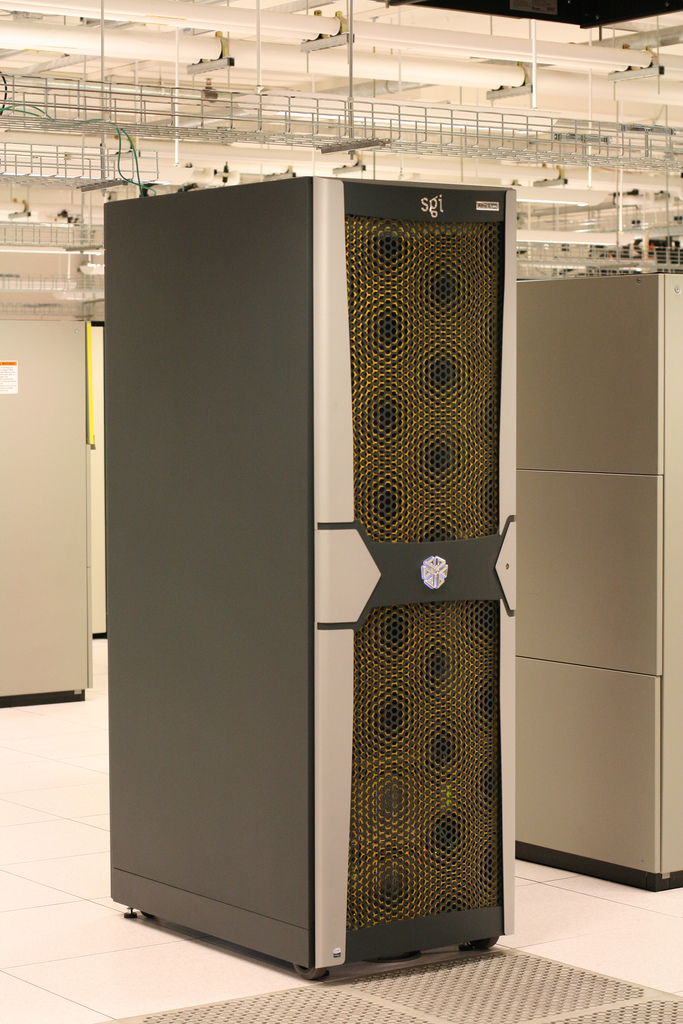
\includegraphics[height=2.7in]{tallbighouse} \end{center}
   \end{column}
   \end{columns}
  \end{frame}
% vislab
\begin{frame}{Hardware: 3dlab}
 \begin{center}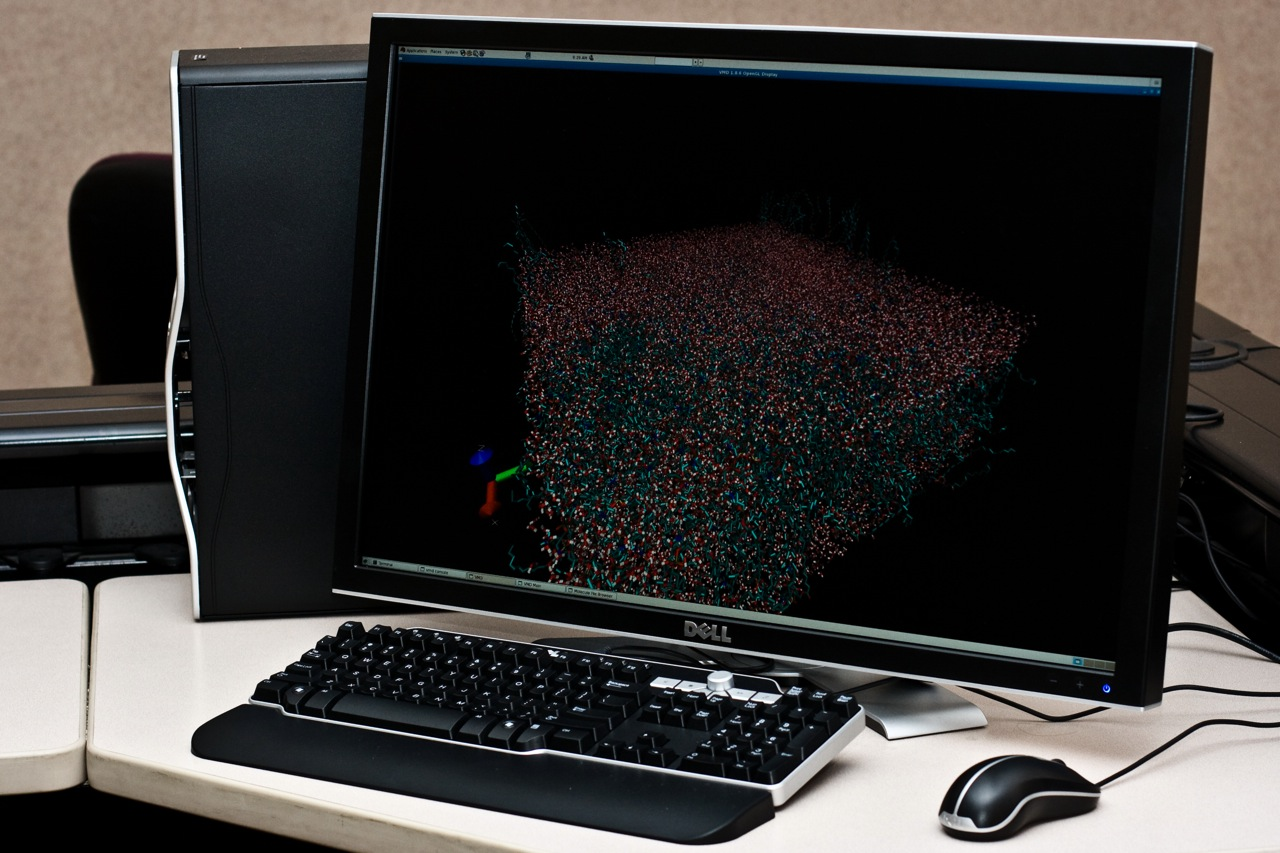
\includegraphics[height=2.0in]{3dlab}\end{center}
  \begin{itemize}
   \item VMD Visual Molecular Dynamics
   \note[item]{VMD \url{http://www.ks.uiuc.edu/Research/vmd/}}
   \item Visit
   \note[item]{Visit \url{https://wci.llnl.gov/codes/visit/}}
   \item IDL Interactive Data Language
   \note[item]{IDL \url{http://www.ittvis.com/idl/}}
   \item Has /nobackup mounted
  \end{itemize}
\end{frame}
% stroage
\begin{frame}{Storage}
 \begin{columns}[c]
 \begin{column}{7cm}
 \begin{block}{/home}
  \begin{itemize}
   \item 6TB total size
   \item 40GB quota per user
   \item Reliable but slow
   \item Only for current jobs
  \end{itemize}
 \end{block}
 \begin{block}{/nobackup}
  \begin{itemize}
   \item Fast and supports MPI-IO
   \item 73TB total size
   \item No quotas
   \item Only for current jobs
   \item \texttt{mkdir /nobackup/\$USER}
  \end{itemize}
 \end{block}
 \end{column}
 \begin{column}{5cm}
  \begin{center}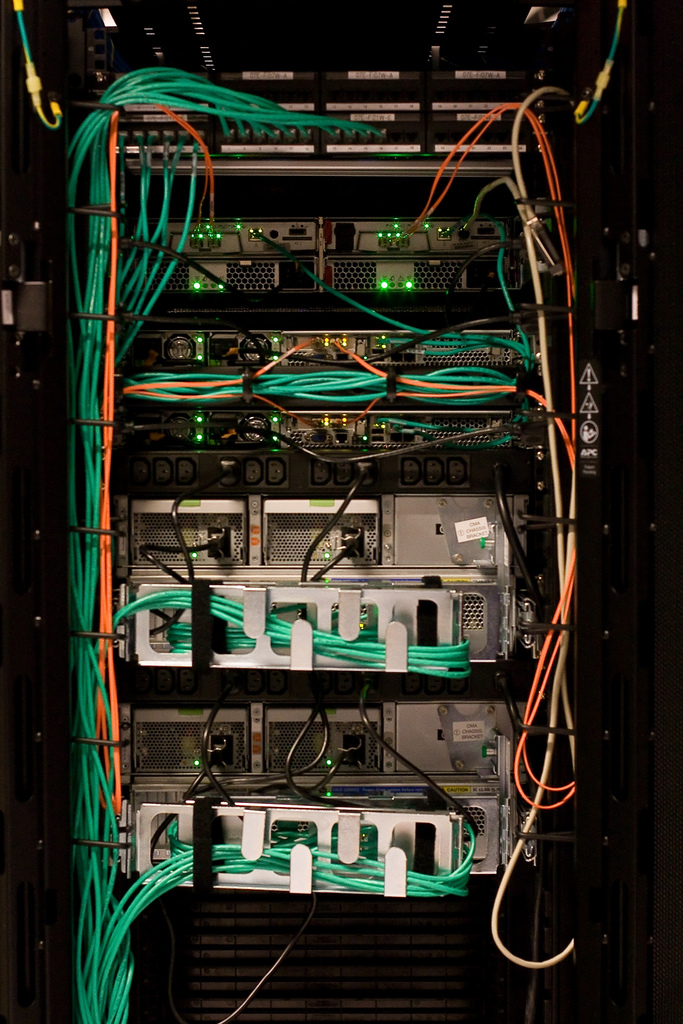
\includegraphics[height=2.7in]{Lustre}\end{center}
 \end{column}
\end{columns}
\note{
Both filesystems are shared on all CAC systems.
\url{http://cac.engin.umich.edu/resources/storage/lustre.html}
\\
For /nobackup user directories have to be created by the user \texttt{mkdir /nobackup/\$USER}.  All users are logged into /home by default. \\

Users can check their quota useage on home with \texttt{quota}.\\
Users can also see their use of /nobackup with: \texttt{lfs quota /nobackup/}\\

\texttt{/home} provides snapshots, a readonly view of your directory at a point in time, this allows recovery of modified/deleted files, but is not a backup for defence against hardware failure.  \\
Snapshots are located at \texttt{/home/.ckpt/}.
} %end note
\end{frame}
  
%default software  
  \subsection {Default Software}
  \begin{frame}{Software}
    \begin{block}{Nyx Defaults}
    \begin{itemize}
      \item OpenMPI
      \item PGI Compilers
    \end{itemize}
    \end{block}
    \begin{block}{Bighouse Defaults}
    \begin{itemize}
      \item Message Passing Toolkit (MPT)
      \item Intel Compilers
    \end{itemize}
    \end{block}
  \end{frame}

  \begin{frame}{Common Software}
   \begin{block}{Common Software}
    \begin{itemize}
     \item PBS Commands
     \item High Performance Math Libraries
     \item Unix/GNU Tools
     \item gcc/g++
    \end{itemize}
   \end{block}
  \end{frame}

%modules
\begin{frame}{Manipulating Software}
  All CAC systems use \texttt{modules} to control software. Users \textit{can} and \textit{should} write their own modules if needed.
  \begin{block}{module commands}
  \begin{itemize}
    \item \texttt{module list} \\ Show loaded modules
    \item \texttt{module load \textit{modulename}} \\  Load \textit{modulename} for use
    \item \texttt{module avail \textit{modulename}} \\ Show available versions of module \textit{modulename}
    \item \texttt{module rm \textit{modulename}} \\  Remove currently loaded module
  \end{itemize}
  \end{block}
  \note[item]{Show Example}
\end{frame}
\begin{frame}{Module Fun}
  \begin{block}{Module Customization}
  \begin{itemize}
  \item \texttt{\~{}/privatemodules/default}
   \\    Allows users to change their default modules.
  \item \texttt{\~{}/privatemodules/\textit{module/version}}
   \\    Holds user created module
  \item \texttt{man modulefile}
  \end{itemize}
  \note[item]{example using fftw follows}
  \end{block}
\end{frame}
\begin{frame}{Module Example}
 \begin{block}{Module Example}
  \begin{itemize}
    \item<1-> List Loaded Modules
         \\ \texttt{module list}
    \item<2-> Show All Modules
         \\ \texttt{module avail}
    \item<3-> Show All Versions of fftw
         \\ \texttt{module avail fftw}
    \item<4-> Load FFTW
         \\ \texttt{module load fftw}
    \item<5-> Show Variables defined by FFTW 
         \\ \texttt{module show fftw}
         \\ \texttt{echo \$FFTW\_LINK}
  \end{itemize}
 \end{block}
\end{frame}
 
%next section how to compile code  

  \section{Mechanics: Usage}
  \subsection{Compiling programs}
  \begin{frame}{Tools}
   \begin{block}{Tools}
    \begin{itemize}
    \item<1- > All of the standard GNU/Linux tools are also available: \texttt{make},
      \texttt{autoconf}, \texttt{awk}, \texttt{sed}, \texttt{Perl}, \texttt{Python},
    \item<2- > We support \texttt{emacs}, \texttt{vi\{m\}}, and \texttt{nano} (a 
      \texttt{pico}-like editor) on the clusters.
      etc.
    \item<3-| alert@1-> Only use \texttt{notepad} on Windows!
    \item<3-| alert@1-> If made on windows fix with \texttt{dos2unix filename}
    \end{itemize}
   \end{block}
  \end{frame}
%compile code
  \begin{frame}{Compile Code}
   \note[item] { The following applies to the default modules}
   \begin{block}{Nyx}
   \begin{itemize}
    \item Use: \texttt{mpicc, mpiCC, mpif90} for MPI code
    \item Use: \texttt{pgcc, pgCC, pgf90} with \texttt{-mp} for OpenMP Code
   \end{itemize}
   \end{block}
   \begin{block}{Bighouse}
    \begin{itemize}
     \item Use: \texttt{icc, icpc, ifort} with \texttt{-lmpi} for MPI code
     \item Use: \texttt{icc, icpc, ifort} with \texttt{-openmp} for OpenMP code
    \end{itemize}
   \end{block}
  \end{frame}
\begin{frame}{Compile Example}
 Copy Code: \texttt{cp \~{}brockp/cac-intro-code.tar.gz \~{}} 
 \\ \texttt{tar -xzvf cac-intro-code.tar.gz}  \\ \texttt{cd \~{}/cac-intro-code}
 \begin{block}{Serial Code}
  \begin{itemize}
   \item Fortran 90
         \\ \texttt{pgf90 -fast -o f90hello helloworld.f90}
   \item C
         \\ \texttt{pgcc -fast -o chello helloworld.c}
  \end{itemize}
 \end{block}
\end{frame}
\begin{frame}{Compile Example Cont'd}
 \begin{block}{MPI Code}
  \begin{itemize}
   \item \texttt{make}
   \item \texttt{mpirun -np 2 c\_ex01}
   \item <2-> Thats it...  Ok not really
   \item <3-> \texttt{make clean}
   \item <3-> \texttt{mpicc -fast -o c\_ex01 c\_ex01.c}
    \note[item]{'man make' Make lets you manage large bits of code. Works for all source types}
  \end{itemize}
 \end{block}
\end{frame}



  \subsection{The Batch System}
  \begin{frame}{Introduction to the PBS Batch System}
   \begin{block}{PBS}
    \begin{itemize}
    \item All access to the compute nodes (everything other than the login node)
      is via the batch system
    \item We use a system called Torque, it is derived from PBS
    \item The batch system controls access to queues
    \item The scheduling (Maui/Moab) system decides if and where jobs can run
    \item<2-> There is a single queue: \texttt{cac}
    \item<3-> Users with private nodes can check their status with \texttt{resinfo.pl -n RESNAME}
    \end{itemize}
   \end{block}
  \end{frame}
  \begin{frame}{Introduction to the PBS Batch System}
   \begin{block}{PBS Files}
    The steps to using the batch system are:
    \begin{enumerate}
    \item Create a batch file: this is a short (5-15 lines) text file with some
      batch commands and the commands to run your program
    \item Submit the file to the batch system
    \item Check on the status of your job
    \item Delete your job if you want to cancel it
    \end{enumerate}
   \end{block}
  \end{frame}
\begin{frame}[fragile]
  \frametitle{Creating a PBS Batch File}
A simple single cpu example
  \begin{semiverbatim}
\uncover<1->{#!/bin/sh}
\uncover<1->{#PBS -N cpu-1}
\uncover<2->{#PBS -l nodes=1,walltime=1:00:00}
\uncover<3->{#PBS -m abe}
\uncover<3->{#PBS -M brockp@umich.edu}
\uncover<4->{#PBS -q route}
\uncover<5->{#PBS -j oe}
\uncover<6->{#PBS -V}
\uncover<7->{cat \$PBS\_NODEFILE}
\uncover<8->{cd \~{}/input1dir/}
\uncover<8->{mcnp5.mpi i=input o=output r=restart}
  \end{semiverbatim}
\end{frame}
\begin{frame}[fragile]
  \frametitle{Creating a PBS Batch File}
  \begin{semiverbatim}  
\uncover{#!/bin/sh}
\uncover{#PBS -N mcnp-8x2}
\uncover{#PBS -l nodes=8:ppn=2,walltime=8:00:00}
\uncover{#PBS -q route}
\uncover{#PBS -M brockp@umich.edu}
\uncover{#PBS -m ae}
\uncover{#PBS -j oe}
\uncover{#PBS -V}
\uncover{cd \$\{HOME\}/input2/}
\uncover{echo "I ran on: "}
\uncover{cat \$PBS\_NODEFILE}
\uncover{mpirun -np 16 mcnp5.mpi i=input2 o=output2 r=restart2}
  \end{semiverbatim}  
 \note[item]{-N sets the job name, can not start with a number}
 \note[item]{-l sets the resources, walltime=HH:MM:SS or walltime=SSSSS Total number of cpus is nodes*ppn which must equal -np. When running under PBS -np is optional. If ommited one rank is started per requested cpu.}
 \note[item]{-q optional: which queue to submit to, use default: \texttt{route}}
 \note[item]{-M Who to email, can be more than one address}
 \note[item]{-m when to email a=abort, b=begin, e=end}
 \note[item]{-j optional: join STDOUT and STDERR default is to not}
 \note[item]{-V Copy submit environment to compute environtment, ALWAYS use this}
 \note{See \texttt{man qsub} for all options}
 \note{Example pbs file included with example codes \texttt{run}}
\end{frame}
\begin{frame}[fragile]
  \frametitle{Submitting, Checking, and Deleting Batch Jobs}
  \begin{itemize}
  \item<1-> After you create your PBS script, you need to submit it:\\
  \tiny
\begin{semiverbatim}
$ qsub  mcnp.q 
542.nyx-login.engin.umich.edu
\end{semiverbatim}
\normalsize
  \item<2-> After you submit your script, you can check on the status of your
job:\\
  \tiny
\begin{semiverbatim}
$ qstat -au brockp
nyx-login.engin.umich.edu: 
Job ID               Username Queue    Jobname    SessID NDS   TSK Memory Time  S Time
-------------------- -------- -------- ---------- ------ ----- --- ------ ----- - -----
542.nyx-login.engin. brockp   short    mcnp-8x2     18922     8  --    --  08:00 R 00:00

$ checkjob 542
[... lots of output ...]
\end{semiverbatim}
\normalsize
  \item<3-> If you want to delete your job:\\
\tiny
\begin{semiverbatim}
$ qdel 542
\end{semiverbatim}\normalsize
  \end{itemize}
\end{frame}
\begin{frame}[fragile]
 \frametitle{PBS Email}
PBS will send an email at the start and end of your job if you use the
\texttt{-m} and \texttt{-M} options in your PBS script.  The email after a job
completes successfully looks like:
\tiny
\begin{verbatim}
Date: Sun, 30 Apr 2006 12:50:17 -0400
From: adm <adm@nyx-login.engin.umich.edu>
To: "Palen, Brock E" <brockp@umich.edu>
Subject: PBS JOB 542.nyx-login.engin.umich.edu
----------------------------------------

PBS Job Id: 542.nyx-login.engin.umich.edu
Job Name:   mcnp-8x2
Execution terminated
Exit_status=0
resources_used.cput=13:17:26
resources_used.mem=1220672kb
resources_used.vmem=11146704kb
resources_used.walltime=00:49:57
\end{verbatim}
\normalsize
\end{frame}

%example
\begin{frame}{PBS Example}
 \begin{block}{PBS Example Job}
  \texttt{cd \~{}/cac-intro-code}
  \\ \texttt{nano run}
  \\ Edit \texttt{\#PBS -M}
  \\ \texttt{Ctl+o}
  \\ \texttt{Ctl+x}
  \\ \texttt{qsub run}
  \note{Please be sure to edit the email address I don't want to be getting all your mail\\}
  \note{Nano is a clone of pico, \^C means Ctl-C, to save \^O to exit \^X}
 \end{block}
\end{frame}
\begin{frame}{Interactive Jobs}
 \begin{block}{Interactive Jobs}
  \uncover<2-> {The CAC has cpus for jobs 15 minutes or less \\}
  \uncover<2-> {These cpus can be used for testing PBS scripts and debugging code \\}
  \uncover<3-> {Interactive jobs allow users to interact with the shell on a remote node \\}
 \end{block}
 \begin{block}{Example}
  \uncover<4-> {\texttt{qsub -I -V -l nodes=2:ppn=2,walltime=15:00 -q cac}}
  \note{Interactive jobs can use X11 forwarding also}
  \note[item]{\texttt{qsub -I -X -V -l nodes=2:ppn=2,walltime=15:00 -q route}}
  \note[item]{Used with ddt our parallel debugger}
 \end{block}
\end{frame}
%preempt jobs
\begin{frame}{Preemptable Jobs}
 \begin{block}{Preempt}
  \begin{itemize}
   \item{Gives fast access to lots of fast cpus}
   \item{Great for hundreds of short jobs}
   \item{Uses Private nodes}
   \item{Read: \url{http://cac.engin.umich.edu/resources/software/pbspreemption.html}}
  \end{itemize}
 \end{block}
 \begin{block}{How to use Preemption}
  \texttt{\#PBS -l nodes=1:ppn=4,}\textbf{qos=preempt}
 \end{block}
\end{frame}

\section{The Scheduler}
\subsection{Understanding the Scheduler}
\begin{frame}{Understanding the Scheduler}
The scheduler determines what jobs can run, when they can run, and where.  There
are many factors that go into the scheduler's decision.
   \begin{block}{Limits and Priority}
    \begin{itemize}
    \item<1-> Limited number jobs eligible for scheduling
    \item<1-> Maximum number of cpus in use by one person: depends on queue
    \item<1-> Maximum number of jobs in the queue at one time: no limit
    \end{itemize}
    \begin{itemize}
    \item<2-> How long you've waited: the longer you wait, the higher your priority
    \item<2-> Your recent usage (fairshare): People with less usage over the past month will have a higher priority than those with a lot of usage

    \note[item]{We can do priorities and limits in private queues as needed for those queues. Limits on User, group, hardware in use, time of use walltime are all options}
    \end{itemize}
   \end{block}
\end{frame}
\begin{frame}{Understanding the Scheduler}
  \begin{itemize}
  \item<1-> Reservations
    \begin{itemize}
    \item<1-> Advance reservations: holds nodes for users or groups
    \item<1-> Job reservations: scheduler will reserve nodes for the next
several jobs in each queue
    \end{itemize}
  \item<2-> Backfill
    \begin{itemize}
    \item<2-> If the reservations leave holes in the schedule, they may be
filled by short jobs that otherwise would have waited.\\
	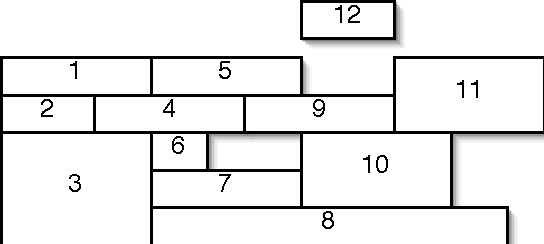
\includegraphics{job-grid}
    \end{itemize}
  \end{itemize}
\end{frame}
\subsection{Scheduler Commands}
\begin{frame}{Understanding the Scheduler}
There are several commands that can give you insight into the scheduler's
decisions.
\begin{itemize}
\item \texttt{showq} --- shows the state of the queue at that moment in time,
showing the running jobs in order of soonest to finish to longest to finish; the
idle jobs in order of priority; and the blocked jobs in the order they were
submitted
\item \texttt{diagnose -p} --- shows the factors that go into computing the
priority for all of the idle jobs
\item \texttt{checkjob \textit{jobnumber}} --- for idle jobs this will show why
the job can't start
\item \texttt{showstart \textit{jobnumber}} --- this makes a (poor) estimate of
when the job will start
\end{itemize}
\end{frame}
\section{Summary}
\subsection{Resources and Access}
\begin{frame}{Summary}
 \begin{block}{Summary}
 \begin{itemize}
  \item Resources
   \begin{itemize}
    \item Lots of cpus
    \item A reasonable amount of software
    \item Watch or subscribe to \url{http://cac.engin.umich.edu} for updates
   \end{itemize}
   \item Access
    \begin{itemize}
     \item All access is via the SSH family of commands: \texttt{ssh},
\texttt{sftp}, \texttt{scp}
     \item There are lots of clients for these commands for the different
platforms
     \item There is no graphical access, everything is via the command line
    \end{itemize}
 \end{itemize}
 \end{block}
\end{frame}
\subsection{Job Management}
\begin{frame}{Summary}
 \begin{block}{Summary Cont'd}
 \begin{itemize}
   \item Job Submission
     \begin{itemize}
     \item Every job needs a PBS script file
     \item Two most important commands: \texttt{qsub} and \texttt{qstat -au \textit{uniqname}}
     \end{itemize}
   \item Job Scheduling
     \begin{itemize}
     \item Scheduling depends on a lot of factors, it is best to submit jobs and let the
scheduler optimize for their start.
     \end{itemize}
 \end{itemize}
 \end{block}
\end{frame}
\subsection{Contact}
\begin{frame}{Summary}
 \begin{block}{Summary Con'd}
 \begin{itemize}
 \item News: \url{http://cac.engin.umich.edu}
   \begin{itemize}
    \item RSS feed
    \item New of changes, outages, other pertinent piece of information
   \end{itemize}
  \item Contact: \url{cac-support@umich.edu}
   \begin{itemize}
    \item Questions or concerns should be sent here (not to an individual) since
this is read by six people.  The odds of a quick reply are best this way.
    \item We aren't parallel programmers, but we'll do what we can to help.
   \end{itemize}
 \end{itemize}
 \end{block}
 \begin{block}{Survey}
    \url{https://www.engin.umich.edu/form/exit09}
 \end{block}
\end{frame}
\end{document}
